\documentclass[../../../main]{subfiles}
\begin{document}
\subsubsection{Qudrature Decoder introduction}
The Quadrature Decoder is used to interprete the position of the system's motors using the signals from the two enocders, each  mounted on motor. This subsection will introduce a little theory of a both Qudrature Decoder and encoder and how the Quadrature decoder has been implementated on the FPGA.
\subsubsection{Quadrature Encoder}
\label{sub:Theory}

First, in order to understand the implementation of the Quadrature Decoder on the FPGA, a small explanation of how a Quadrature Encoder works is needed. \\
A Quadrature Encoder uses two channels to sense the position of, typically, a rotating disk/shaft or a linear strip. The disk or strip has two paths on it, positioned 90 degresse out of phase of each other, see figure \ref{rotary_encoder} for a rotary encoder and figure \ref{channels_1} for a strip encoder. Statinoary sensores are typically placed on top of the encoder, so when a track moves in relation to a sensor, it outputs a logic high or low output signal depending on what part of the track is visible to the sensor. An encoder has two output signals, one for each channel, typically called A and B, see figure \ref{channels_1} for a representation of those for both encoder types. This two signals, A and B, is what the decoder uses to determine the position of the encoder.

\begin{figure}[H]
  
\includegraphics[width = \textwidth]{\main/afsnit/system_implementation/Quadraturdecoder/pictures/encoder.png}
  \caption{The figure shows the tracks of a rotary encoder.}
  \label{rotary_encoder}
\end{figure}

\begin{figure}[H]
  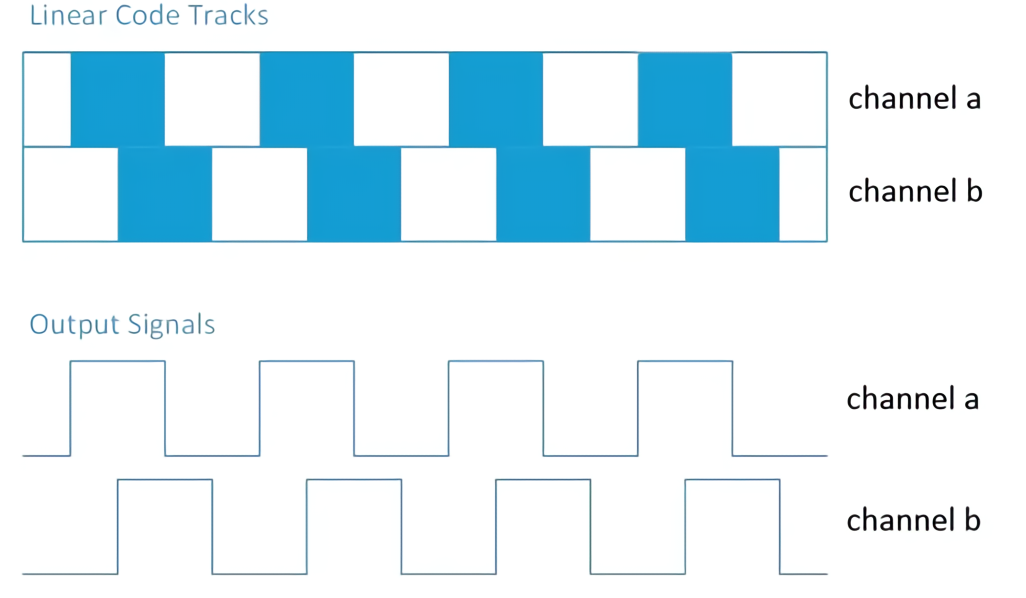
\includegraphics[width = \textwidth]{\main/afsnit/system_implementation/Quadraturdecoder/pictures/channels.png}
  \caption{The upper figure a Linear encoder and the lower figure shows the output of both a rotary and linary encoder}
  \label{channels_1}
\end{figure}
\footnote{https://www.digikey.com/eewiki/pages/viewpage.action?pageId=62259228 - kilden}

\subsubsection{Decoder principle}
The basic principle of a Quadrature Decoder is for it to decode the two output signals the encoder produces and return a position. The idea is to observe the both the encoders outputs. By counting the transitions from high to low and low to high on just one of the outputs, it can be determined how far the encoder has rotated. However, by adding the second output, the direction of the encoder can be computed as well as adding a higher resolution to the position. The encoder used in the project is a rotary encoder with a resolution of 360\footnote{See datasheet x}, which means that a Quadrature Decoder will count 360 "ticks" per shaft turn. This resolution and rotation can not be mapped directly to the system itself as its motors are geared. The motors do three full rotations of their shafts before the system itself has completed a full rotation. Hence the resolution for the system is 1080. This is very useful, since it gives a $\frac{1}{3}$ of a degrees position precision.
\subsubsection{Statemachine}
To use the transitions between encoder output A and output B, a truth table of every possible combination of the two singals must be computed. As mentioned in system design it is necessary to include a third signal called "return to home" in order to reset the position counter if a new reference point is desired. The truth table including all three signals is shown in figure \ref{fig:truth_table}.
\begin{figure}[H]
  \begin{tabular}{|c | c | c | c | c | c |c |}
  \hline
   A\_prev & A\_new & B\_prev & B\_new & Reset & Direction & Position \\
   \hline
   0 & 1 & 0 & 0 & 1 & Forward & + 1 \\
   1 & 1 & 0 & 1 & 1 & Forward & + 1 \\
   1 & 0 & 1 & 1 & 1 & Forward & + 1 \\
   0 & 0 & 1 & 0 & 1 & Forward & + 1 \\
   0 & 0 & 0 & 1 & 1 & Backward & - 1 \\
   1 & 0 & 0 & 0 & 1 & Backward & - 1 \\
   0 & 1 & 1 & 1 & 1 & Backward & - 1 \\
   1 & 1 & 1 & 0 & 1 & Backward & - 1 \\
   x & x & x & x & 0 & No change &  0 \\
   \hline
  \end{tabular}
  \caption{This figure shows the truth table for the Quadrature decoder}
  \label{fig:truth_table}
\end{figure}
The truth table shows nine possible scenarios that can occur from tracking the transistions of the outputs. Four of these results in a forward direction and the counter will increment, four scenarios results in a backwards direction and the counter will decrement. The last scenario occurs if the return to home flag is set low\footnote{Return to home is implemented as active low, as can be observed in the truth table \ref{fig:truth_table}.}, and the counter is set to zero regardless of what it was on before. From these observations a state machine containing 6 states has been computed. The states are: AB\_low with the gray code $001$\footnote{The first digit is signal A, second is signal B and thrid is the reset signal}, AB\_high with gray code $111$, A\_high with gray code $101$, B\_high with gray code $011$, undefined and reset $xx0$. The undefined state is purely for debugging purposes used if an error with the signal A and B ocurs. A potential error could be if the state is currently AB\_low the gray code can not be $111$ in the next instance. This would mean that both signals changed at the same time. The decoder works by first initialalizing and go to a state depending on the level of signal A and B. The decoder will when use the debounced signals to see what state will be the next to switch to. If the starting state is AB\_low, there is three correct outcomes: the reset signal goes low and the counter will go to zero. the signal A goes high whcih means that the state will change to

\begin{figure}[H]
    \centering
    \def\svgwidth{\columnwidth}
    \input{\main/afsnit/system_implementation/Quadraturdecoder/pictures/decoder_state.pdf_tex}
\end{figure}

The singals are all debounced to ensure that noise is not altering the position.
\end{document}
